%% bare_jrnl.tex
%% V1.4b
%% 2015/08/26
%% by Michael Shell
%% see http://www.michaelshell.org/
%% for current contact information.
%%
%% This is a skeleton file demonstrating the use of IEEEtran.cls
%% (requires IEEEtran.cls version 1.8b or later) with an IEEE
%% journal paper.
%%
%% Support sites:
%% http://www.michaelshell.org/tex/ieeetran/
%% http://www.ctan.org/pkg/ieeetran
%% and
%% http://www.ieee.org/

%%*************************************************************************
%% Legal Notice:
%% This code is offered as-is without any warranty either expressed or
%% implied; without even the implied warranty of MERCHANTABILITY or
%% FITNESS FOR A PARTICULAR PURPOSE!
%% User assumes all risk.
%% In no event shall the IEEE or any contributor to this code be liable for
%% any damages or losses, including, but not limited to, incidental,
%% consequential, or any other damages, resulting from the use or misuse
%% of any information contained here.
%%
%% All comments are the opinions of their respective authors and are not
%% necessarily endorsed by the IEEE.
%%
%% This work is distributed under the LaTeX Project Public License (LPPL)
%% ( http://www.latex-project.org/ ) version 1.3, and may be freely used,
%% distributed and modified. A copy of the LPPL, version 1.3, is included
%% in the base LaTeX documentation of all distributions of LaTeX released
%% 2003/12/01 or later.
%% Retain all contribution notices and credits.
%% ** Modified files should be clearly indicated as such, including  **
%% ** renaming them and changing author support contact information. **
%%*************************************************************************


% *** Authors should verify (and, if needed, correct) their LaTeX system  ***
% *** with the testflow diagnostic prior to trusting their LaTeX platform ***
% *** with production work. The IEEE's font choices and paper sizes can   ***
% *** trigger bugs that do not appear when using other class files.       ***                          ***
% The testflow support page is at:
% http://www.michaelshell.org/tex/testflow/



\documentclass[a4paper,journal]{IEEEtran}
%
% If IEEEtran.cls has not been installed into the LaTeX system files,
% manually specify the path to it like:
% \documentclass[journal]{../sty/IEEEtran}





% Some very useful LaTeX packages include:
% (uncomment the ones you want to load)


% *** MISC UTILITY PACKAGES ***
%
%\usepackage{ifpdf}
% Heiko Oberdiek's ifpdf.sty is very useful if you need conditional
% compilation based on whether the output is pdf or dvi.
% usage:
% \ifpdf
%   % pdf code
% \else
%   % dvi code
% \fi
% The latest version of ifpdf.sty can be obtained from:
% http://www.ctan.org/pkg/ifpdf
% Also, note that IEEEtran.cls V1.7 and later provides a builtin
% \ifCLASSINFOpdf conditional that works the same way.
% When switching from latex to pdflatex and vice-versa, the compiler may
% have to be run twice to clear warning/error messages.






% *** CITATION PACKAGES ***
%
%\usepackage{cite}
% cite.sty was written by Donald Arseneau
% V1.6 and later of IEEEtran pre-defines the format of the cite.sty package
% \cite{} output to follow that of the IEEE. Loading the cite package will
% result in citation numbers being automatically sorted and properly
% "compressed/ranged". e.g., [1], [9], [2], [7], [5], [6] without using
% cite.sty will become [1], [2], [5]--[7], [9] using cite.sty. cite.sty's
% \cite will automatically add leading space, if needed. Use cite.sty's
% noadjust option (cite.sty V3.8 and later) if you want to turn this off
% such as if a citation ever needs to be enclosed in parenthesis.
% cite.sty is already installed on most LaTeX systems. Be sure and use
% version 5.0 (2009-03-20) and later if using hyperref.sty.
% The latest version can be obtained at:
% http://www.ctan.org/pkg/cite
% The documentation is contained in the cite.sty file itself.






% *** GRAPHICS RELATED PACKAGES ***
%
\ifCLASSINFOpdf
  \usepackage[pdftex]{graphicx}
  % declare the path(s) where your graphic files are
  \graphicspath{{../diagram_dst/}}
  % and their extensions so you won't have to specify these with
  % every instance of \includegraphics
  \DeclareGraphicsExtensions{.pdf,.jpeg,.png}
\else
  % or other class option (dvipsone, dvipdf, if not using dvips). graphicx
  % will default to the driver specified in the system graphics.cfg if no
  % driver is specified.
  % \usepackage[dvips]{graphicx}
  % declare the path(s) where your graphic files are
  % \graphicspath{{../eps/}}
  % and their extensions so you won't have to specify these with
  % every instance of \includegraphics
  % \DeclareGraphicsExtensions{.eps}
\fi
% graphicx was written by David Carlisle and Sebastian Rahtz. It is
% required if you want graphics, photos, etc. graphicx.sty is already
% installed on most LaTeX systems. The latest version and documentation
% can be obtained at:
% http://www.ctan.org/pkg/graphicx
% Another good source of documentation is "Using Imported Graphics in
% LaTeX2e" by Keith Reckdahl which can be found at:
% http://www.ctan.org/pkg/epslatex
%
% latex, and pdflatex in dvi mode, support graphics in encapsulated
% postscript (.eps) format. pdflatex in pdf mode supports graphics
% in .pdf, .jpeg, .png and .mps (metapost) formats. Users should ensure
% that all non-photo figures use a vector format (.eps, .pdf, .mps) and
% not a bitmapped formats (.jpeg, .png). The IEEE frowns on bitmapped formats
% which can result in "jaggedy"/blurry rendering of lines and letters as
% well as large increases in file sizes.
%
% You can find documentation about the pdfTeX application at:
% http://www.tug.org/applications/pdftex





% *** MATH PACKAGES ***
%
%\usepackage{amsmath}
% A popular package from the American Mathematical Society that provides
% many useful and powerful commands for dealing with mathematics.
%
% Note that the amsmath package sets \interdisplaylinepenalty to 10000
% thus preventing page breaks from occurring within multiline equations. Use:
%\interdisplaylinepenalty=2500
% after loading amsmath to restore such page breaks as IEEEtran.cls normally
% does. amsmath.sty is already installed on most LaTeX systems. The latest
% version and documentation can be obtained at:
% http://www.ctan.org/pkg/amsmath





% *** SPECIALIZED LIST PACKAGES ***
%
%\usepackage{algorithmic}
% algorithmic.sty was written by Peter Williams and Rogerio Brito.
% This package provides an algorithmic environment fo describing algorithms.
% You can use the algorithmic environment in-text or within a figure
% environment to provide for a floating algorithm. Do NOT use the algorithm
% floating environment provided by algorithm.sty (by the same authors) or
% algorithm2e.sty (by Christophe Fiorio) as the IEEE does not use dedicated
% algorithm float types and packages that provide these will not provide
% correct IEEE style captions. The latest version and documentation of
% algorithmic.sty can be obtained at:
% http://www.ctan.org/pkg/algorithms
% Also of interest may be the (relatively newer and more customizable)
% algorithmicx.sty package by Szasz Janos:
% http://www.ctan.org/pkg/algorithmicx
\usepackage[inline]{enumitem}


% *** ALIGNMENT PACKAGES ***
%
%\usepackage{array}
% Frank Mittelbach's and David Carlisle's array.sty patches and improves
% the standard LaTeX2e array and tabular environments to provide better
% appearance and additional user controls. As the default LaTeX2e table
% generation code is lacking to the point of almost being broken with
% respect to the quality of the end results, all users are strongly
% advised to use an enhanced (at the very least that provided by array.sty)
% set of table tools. array.sty is already installed on most systems. The
% latest version and documentation can be obtained at:
% http://www.ctan.org/pkg/array


% IEEEtran contains the IEEEeqnarray family of commands that can be used to
% generate multiline equations as well as matrices, tables, etc., of high
% quality.




% *** SUBFIGURE PACKAGES ***
%\ifCLASSOPTIONcompsoc
%  \usepackage[caption=false,font=normalsize,labelfont=sf,textfont=sf]{subfig}
%\else
%  \usepackage[caption=false,font=footnotesize]{subfig}
%\fi
% subfig.sty, written by Steven Douglas Cochran, is the modern replacement
% for subfigure.sty, the latter of which is no longer maintained and is
% incompatible with some LaTeX packages including fixltx2e. However,
% subfig.sty requires and automatically loads Axel Sommerfeldt's caption.sty
% which will override IEEEtran.cls' handling of captions and this will result
% in non-IEEE style figure/table captions. To prevent this problem, be sure
% and invoke subfig.sty's "caption=false" package option (available since
% subfig.sty version 1.3, 2005/06/28) as this is will preserve IEEEtran.cls
% handling of captions.
% Note that the Computer Society format requires a larger sans serif font
% than the serif footnote size font used in traditional IEEE formatting
% and thus the need to invoke different subfig.sty package options depending
% on whether compsoc mode has been enabled.
%
% The latest version and documentation of subfig.sty can be obtained at:
% http://www.ctan.org/pkg/subfig




% *** FLOAT PACKAGES ***
%
%\usepackage{fixltx2e}
% fixltx2e, the successor to the earlier fix2col.sty, was written by
% Frank Mittelbach and David Carlisle. This package corrects a few problems
% in the LaTeX2e kernel, the most notable of which is that in current
% LaTeX2e releases, the ordering of single and double column floats is not
% guaranteed to be preserved. Thus, an unpatched LaTeX2e can allow a
% single column figure to be placed prior to an earlier double column
% figure.
% Be aware that LaTeX2e kernels dated 2015 and later have fixltx2e.sty's
% corrections already built into the system in which case a warning will
% be issued if an attempt is made to load fixltx2e.sty as it is no longer
% needed.
% The latest version and documentation can be found at:
% http://www.ctan.org/pkg/fixltx2e


%\usepackage{stfloats}
% stfloats.sty was written by Sigitas Tolusis. This package gives LaTeX2e
% the ability to do double column floats at the bottom of the page as well
% as the top. (e.g., "\begin{figure*}[!b]" is not normally possible in
% LaTeX2e). It also provides a command:
%\fnbelowfloat
% to enable the placement of footnotes below bottom floats (the standard
% LaTeX2e kernel puts them above bottom floats). This is an invasive package
% which rewrites many portions of the LaTeX2e float routines. It may not work
% with other packages that modify the LaTeX2e float routines. The latest
% version and documentation can be obtained at:
% http://www.ctan.org/pkg/stfloats
% Do not use the stfloats baselinefloat ability as the IEEE does not allow
% \baselineskip to stretch. Authors submitting work to the IEEE should note
% that the IEEE rarely uses double column equations and that authors should try
% to avoid such use. Do not be tempted to use the cuted.sty or midfloat.sty
% packages (also by Sigitas Tolusis) as the IEEE does not format its papers in
% such ways.
% Do not attempt to use stfloats with fixltx2e as they are incompatible.
% Instead, use Morten Hogholm'a dblfloatfix which combines the features
% of both fixltx2e and stfloats:
%
% \usepackage{dblfloatfix}
% The latest version can be found at:
% http://www.ctan.org/pkg/dblfloatfix




%\ifCLASSOPTIONcaptionsoff
%  \usepackage[nomarkers]{endfloat}
% \let\MYoriglatexcaption\caption
% \renewcommand{\caption}[2][\relax]{\MYoriglatexcaption[#2]{#2}}
%\fi
% endfloat.sty was written by James Darrell McCauley, Jeff Goldberg and
% Axel Sommerfeldt. This package may be useful when used in conjunction with
% IEEEtran.cls'  captionsoff option. Some IEEE journals/societies require that
% submissions have lists of figures/tables at the end of the paper and that
% figures/tables without any captions are placed on a page by themselves at
% the end of the document. If needed, the draftcls IEEEtran class option or
% \CLASSINPUTbaselinestretch interface can be used to increase the line
% spacing as well. Be sure and use the nomarkers option of endfloat to
% prevent endfloat from "marking" where the figures would have been placed
% in the text. The two hack lines of code above are a slight modification of
% that suggested by in the endfloat docs (section 8.4.1) to ensure that
% the full captions always appear in the list of figures/tables - even if
% the user used the short optional argument of \caption[]{}.
% IEEE papers do not typically make use of \caption[]'s optional argument,
% so this should not be an issue. A similar trick can be used to disable
% captions of packages such as subfig.sty that lack options to turn off
% the subcaptions:
% For subfig.sty:
% \let\MYorigsubfloat\subfloat
% \renewcommand{\subfloat}[2][\relax]{\MYorigsubfloat[]{#2}}
% However, the above trick will not work if both optional arguments of
% the \subfloat command are used. Furthermore, there needs to be a
% description of each subfigure *somewhere* and endfloat does not add
% subfigure captions to its list of figures. Thus, the best approach is to
% avoid the use of subfigure captions (many IEEE journals avoid them anyway)
% and instead reference/explain all the subfigures within the main caption.
% The latest version of endfloat.sty and its documentation can obtained at:
% http://www.ctan.org/pkg/endfloat
%
% The IEEEtran \ifCLASSOPTIONcaptionsoff conditional can also be used
% later in the document, say, to conditionally put the References on a
% page by themselves.




% *** PDF, URL AND HYPERLINK PACKAGES ***
%
%\usepackage{url}
% url.sty was written by Donald Arseneau. It provides better support for
% handling and breaking URLs. url.sty is already installed on most LaTeX
% systems. The latest version and documentation can be obtained at:
% http://www.ctan.org/pkg/url
% Basically, \url{my_url_here}.




% *** Do not adjust lengths that control margins, column widths, etc. ***
% *** Do not use packages that alter fonts (such as pslatex).         ***
% There should be no need to do such things with IEEEtran.cls V1.6 and later.
% (Unless specifically asked to do so by the journal or conference you plan
% to submit to, of course. )


% correct bad hyphenation here
\hyphenation{op-tical net-works semi-conduc-tor}


\begin{document}
%
% paper title
% Titles are generally capitalized except for words such as a, an, and, as,
% at, but, by, for, in, nor, of, on, or, the, to and up, which are usually
% not capitalized unless they are the first or last word of the title.
% Linebreaks \\ can be used within to get better formatting as desired.
% Do not put math or special symbols in the title.
\title{Technical Specification\\for an Online Technology Store}
%
%
% author names and IEEE memberships
% note positions of commas and nonbreaking spaces ( ~ ) LaTeX will not break
% a structure at a ~ so this keeps an author's name from being broken across
% two lines.
% use \thanks{} to gain access to the first footnote area
% a separate \thanks must be used for each paragraph as LaTeX2e's \thanks
% was not built to handle multiple paragraphs
%

\author{
%Michael~Shell,~\IEEEmembership{Member,~IEEE,}
%John~Doe,~\IEEEmembership{Fellow,~OSA,}
%and~Jane~Doe,~\IEEEmembership{Life~Fellow,~IEEE}% <-this % stops a space
Emre~Özcan,
Eren~Gökçe,
Melisa~Uyar,
Muhammet~Berk~Can,
Oğuz~Anıl~Ateş%
\thanks{All authors were with the Department of Computer Engineering,
Manisa Celâl Bayar University, 45140 Manisa, Türkiye.}% <-this % stops a space
\thanks{Manuscript from December 1, 2024.}% <-this % stops a space
}

% note the % following the last \IEEEmembership and also \thanks -
% these prevent an unwanted space from occurring between the last author name
% and the end of the author line. i.e., if you had this:
%
% \author{....lastname \thanks{...} \thanks{...} }
%                     ^------------^------------^----Do not want these spaces!
%
% a space would be appended to the last name and could cause every name on that
% line to be shifted left slightly. This is one of those "LaTeX things". For
% instance, "\textbf{A} \textbf{B}" will typeset as "A B" not "AB". To get
% "AB" then you have to do: "\textbf{A}\textbf{B}"
% \thanks is no different in this regard, so shield the last } of each \thanks
% that ends a line with a % and do not let a space in before the next \thanks.
% Spaces after \IEEEmembership other than the last one are OK (and needed) as
% you are supposed to have spaces between the names. For what it is worth,
% this is a minor point as most people would not even notice if the said evil
% space somehow managed to creep in.



% The paper headers
%\markboth{Journal of \LaTeX\ Class Files,~Vol.~14, No.~8, August~2015}%
%{Shell \MakeLowercase{\textit{et al.}}: Bare Demo of IEEEtran.cls for IEEE Journals}
\markboth%
{December~2024}%
{Technical Specification for an Online Technology Store}
% The only time the second header will appear is for the odd numbered pages
% after the title page when using the twoside option.
%
% *** Note that you probably will NOT want to include the author's ***
% *** name in the headers of peer review papers.                   ***
% You can use \ifCLASSOPTIONpeerreview for conditional compilation here if
% you desire.




% If you want to put a publisher's ID mark on the page you can do it like
% this:
%\IEEEpubid{0000--0000/00\$00.00~\copyright~2015 IEEE}
% Remember, if you use this you must call \IEEEpubidadjcol in the second
% column for its text to clear the IEEEpubid mark.



% use for special paper notices
%\IEEEspecialpapernotice{(Invited Paper)}




% make the title area
\maketitle

% As a general rule, do not put math, special symbols or citations
% in the abstract or keywords.
\begin{abstract}
% TODO: Write the abstract.
The abstract goes here.
\end{abstract}

% Note that keywords are not normally used for peerreview papers.
% index terms, keywords
%\begin{IEEEkeywords}
%IEEE, IEEEtran, journal, \LaTeX, paper, template.
%\end{IEEEkeywords}






% For peer review papers, you can put extra information on the cover
% page as needed:
% \ifCLASSOPTIONpeerreview
% \begin{center} \bfseries EDICS Category: 3-BBND \end{center}
% \fi
%
% For peerreview papers, this IEEEtran command inserts a page break and
% creates the second title. It will be ignored for other modes.
\IEEEpeerreviewmaketitle



\section{Introduction}
% The very first letter is a 2 line initial drop letter followed
% by the rest of the first word in caps.
%
% form to use if the first word consists of a single letter:
% \IEEEPARstart{A}{demo} file is ....
%
% form to use if you need the single drop letter followed by
% normal text (unknown if ever used by the IEEE):
% \IEEEPARstart{A}{}demo file is ....
%
% Some journals put the first two words in caps:
% \IEEEPARstart{T}{his demo} file is ....
%
% Here we have the typical use of a "T" for an initial drop letter
% and "HIS" in caps to complete the first word.
% TODO: Write the introduction.
\IEEEPARstart{T}{his} demo file is intended to serve as a ``starter file''
for IEEE journal papers produced under \LaTeX\ using
IEEEtran.cls version 1.8b and later.
% You must have at least 2 lines in the paragraph with the drop letter
% (should never be an issue)
I wish you the best of success.

\hfill mds

\hfill August 26, 2015

% TODO:
% needed in second column of first page if using \IEEEpubid
%\IEEEpubidadjcol

% An example of a floating figure using the graphicx package.
% Note that \label must occur AFTER (or within) \caption.
% For figures, \caption should occur after the \includegraphics.
% Note that IEEEtran v1.7 and later has special internal code that
% is designed to preserve the operation of \label within \caption
% even when the captionsoff option is in effect. However, because
% of issues like this, it may be the safest practice to put all your
% \label just after \caption rather than within \caption{}.
%
% Reminder: the "draftcls" or "draftclsnofoot", not "draft", class
% option should be used if it is desired that the figures are to be
% displayed while in draft mode.
%
%\begin{figure}[!t]
%\centering
%\includegraphics[width=2.5in]{myfigure}
% where an .eps filename suffix will be assumed under latex,
% and a .pdf suffix will be assumed for pdflatex; or what has been declared
% via \DeclareGraphicsExtensions.
%\caption{Simulation results for the network.}
%\label{fig_sim}
%\end{figure}

% Note that the IEEE typically puts floats only at the top, even when this
% results in a large percentage of a column being occupied by floats.


% An example of a double column floating figure using two subfigures.
% (The subfig.sty package must be loaded for this to work.)
% The subfigure \label commands are set within each subfloat command,
% and the \label for the overall figure must come after \caption.
% \hfil is used as a separator to get equal spacing.
% Watch out that the combined width of all the subfigures on a
% line do not exceed the text width or a line break will occur.
%
%\begin{figure*}[!t]
%\centering
%\subfloat[Case I]{\includegraphics[width=2.5in]{box}%
%\label{fig_first_case}}
%\hfil
%\subfloat[Case II]{\includegraphics[width=2.5in]{box}%
%\label{fig_second_case}}
%\caption{Simulation results for the network.}
%\label{fig_sim}
%\end{figure*}
%
% Note that often IEEE papers with subfigures do not employ subfigure
% captions (using the optional argument to \subfloat[]), but instead will
% reference/describe all of them (a), (b), etc., within the main caption.
% Be aware that for subfig.sty to generate the (a), (b), etc., subfigure
% labels, the optional argument to \subfloat must be present. If a
% subcaption is not desired, just leave its contents blank,
% e.g., \subfloat[].


% An example of a floating table. Note that, for IEEE style tables, the
% \caption command should come BEFORE the table and, given that table
% captions serve much like titles, are usually capitalized except for words
% such as a, an, and, as, at, but, by, for, in, nor, of, on, or, the, to
% and up, which are usually not capitalized unless they are the first or
% last word of the caption. Table text will default to \footnotesize as
% the IEEE normally uses this smaller font for tables.
% The \label must come after \caption as always.
%
%\begin{table}[!t]
%% increase table row spacing, adjust to taste
%\renewcommand{\arraystretch}{1.3}
% if using array.sty, it might be a good idea to tweak the value of
% \extrarowheight as needed to properly center the text within the cells
%\caption{An Example of a Table}
%\label{table_example}
%\centering
%% Some packages, such as MDW tools, offer better commands for making tables
%% than the plain LaTeX2e tabular which is used here.
%\begin{tabular}{|c||c|}
%\hline
%One & Two\\
%\hline
%Three & Four\\
%\hline
%\end{tabular}
%\end{table}


% Note that the IEEE does not put floats in the very first column
% - or typically anywhere on the first page for that matter. Also,
% in-text middle ("here") positioning is typically not used, but it
% is allowed and encouraged for Computer Society conferences (but
% not Computer Society journals). Most IEEE journals/conferences use
% top floats exclusively.
% Note that, LaTeX2e, unlike IEEE journals/conferences, places
% footnotes above bottom floats. This can be corrected via the
% \fnbelowfloat command of the stfloats package.

\section{Feasibility Study and Plan}
Our objectives are
\begin{enumerate*}
  \item to develope an online technology store with a robust, user-friendly,
    and secure platform,
  \item to integrate essential functionalities for customers, administrators,
    and external service providers,
  \item to Ensure compliance with modern e-commerce standards, GDPR, and
    accessibility guidelines, and
  \item to follow a modular design approach to enable scalability and
    adaptability for future upgrades.
\end{enumerate*}

We will now discuss the feasibility of the project and the plan to achieve the
objectives.

\subsection{Technical Feasibility}
\begin{itemize}
  \item \textbf{Platform:} Java backend using Spring Boot for RESTful APIs
    ensures scalability and maintainability.
  \item \textbf{Frontend:} Svelte for building a dynamic, responsive, and
    lightweight user interface.
  \item \textbf{Database:} PostgreSQL for reliable and scalable data storage.
  \item \textbf{Testing:} JUnit for unit testing and Maven for dependency
    management.
  \item \textbf{Server:} DigitalOcean provides reliable cloud hosting with
    necessary configurations.
  \item \textbf{Design Tools:} Figma for prototype design ensures stakeholder
    collaboration and UI consistency.
  \item \textbf{Monitoring Tools:} Sentry, Datadog, and New Relic provide robust
    monitoring for performance and error tracking.
\end{itemize}

Our assessment is that this stack is reliable, widely supported, and feasible
for the development team's skill set and project scope.

\subsection{Operational Feasibility}
The proposed system ensures seamless engagement with all stakeholders.
Customers will benefit from an intuitive platform offering secure payment
options and efficient order tracking.
Administrators will have access to robust tools for managing products and
inventory, streamlining operational workflows.
IT support teams will be equipped with comprehensive documentation and training,
enabling them to address technical challenges effectively.

Operational management will leverage GitHub Projects with Kanban methodology,
facilitating effective task tracking and prioritization. Overall, the system's
capabilities are well-aligned with stakeholder requirements, supporting
practical and achievable operational goals.

\subsection{Economic Feasibility}
The initial costs of the project only include server costs from DigitalOcean,
which we will eliminate using the GitHub Student Developer Pack which includes
\$200 free credits for DigitalOcean.

The ongoing costs are monitoring tools, software development kits, and
integrated development environment licenses.
We will mitigate most of these using student plans.
Open-source libraries and tools will be used where available to reduce or
eliminate costs (e.g. PostgreSQL instead of Oracle DB).

\subsection{Project Timeline}
\begin{itemize}
  \item \textbf{Week 1--2:} Requirements gathering and feasibility study.
  \item \textbf{Week 3--4:} System design.
  \item \textbf{Week 5--6:} Development.
    \begin{itemize}
      \item Backend API and database integration.
      \item Frontend implementation and unit tests.
    \end{itemize}
  \item \textbf{Week 6--7:} Testing and debugging.
\end{itemize}

\subsection{Legal and Ethical Feasibility}
GDPR compliance will be ensured by anonymizing user data where possible and
encrypting sensitive information.
Ethical design principles will be used to avoid dark patterns and ensure
accessibility for all users.
All third-party libraries and tools will be properly licensed.

\section{Stakeholders}
We have four types of stakeholders:
\begin{enumerate*}
  \item end users,
  \item system managers,
  \item system owners, and
  \item external stakeholders.
\end{enumerate*}
They will now be discussed in detail.

\subsection{End Users}
End users are the primary stakeholders who will interact with the system.

\subsubsection{Customers}
Customers are individuals who browse, purchase, and manage their accounts and
orders in the system. They rely on a seamless shopping experience, including
secure payments and order tracking.

\subsubsection{Store Administrators}
Store administrators are staff responsible for overseeing the overall platform
operations. They manage inventory, update product listings, handle promotions,
discounts, and oversee pricing strategies. Store administrators ensure that all
data related to products, prices, and stock availability is accurate and
up-to-date.

\subsection{System Managers}
System managers are responsible for maintaining the system's operational
efficiency and ensuring that all components are functioning correctly.

\subsubsection{Customer Support Team}
Customer support agents handle inquiries, resolves complaints, and process
returns and exchanges.
They ensure customer satisfaction by addressing issues such as order delays,
faulty products, and assisting with troubleshooting or product recommendations. 
The support team is crucial for maintaining a positive relationship with
customers.

\subsubsection{IT and Development Team}
The IT and development teams include
developers and engineers responsible for building, maintaining, and updating the
website.
They manage security protocols, ensure smooth operation, and implement
performance enhancements. They address technical issues, perform bug fixes,
and ensure that the platform is scalable to handle growth and fluctuating
demand.

\subsection{System Owners}
System owners are the individuals or entities responsible for the system's
development, maintenance, and overall success.

\subsubsection{Business Owners/Management}
The company's leadership, who oversee the strategic direction and financial
health of the platform.
This could include the CEO or senior management
responsible for setting sales targets, customer engagement strategies, and
long-term goals for platform growth.
They ensure that the platform meets market
trends, optimizes profits, and adheres to corporate objectives.

\subsection{External Stakeholders}
External stakeholders are individuals or entities that interact with the system
but are not directly involved in its day-to-day operations.

\subsubsection{Warehouse and Shipping Partners}
Warehouse and shipping partners include logistics companies or internal shipping
departments that handle the storage, packing, and delivery of products to
customers.
They manage inventory in warehouses, ensure products are shipped within the
expected timeframes, and update the system with tracking information.

\subsubsection{Payment Gateway Providers}
Payment gateway providers are external companies that provide secure payment
processing solutions, such as PayPal, credit card processors, or other regional
payment services.
These providers ensure that customers' financial details are protected and that
transactions are processed securely.

\section{Problems and Mitigations}
\subsection{In the Requirements Elicitation Process}
We have identified
\begin{enumerate*}
  \item \textbf{unclear goals,} and
  \item \textbf{feature creep}
\end{enumerate*}
as potential problems.

Without external feedback, it can be challenging to identify all the critical
requirements, and we might focus too much on secondary features that are not
essential for the core functionality of our system.
\textit{(unclear goals)}

The lack of constraints might cause us to continually expand the scope of the
project, which could delay the launch and increase complexity unnecessarily.
\textit{(feature creep)}

We propose the following mitigations:
\begin{itemize}
  \item \textbf{Clarifying the objectives:}
    We must define clear and concrete project goals from the start and ensure that
    every feature aligns with the broader system objectives.
  \item \textbf{Prioritization of features:}
    We should use a
    prioritization framework like MoSCoW (Must have, Should have, Could have,
    Won't have) to focus only on the features essential to the system’s core
    functionality.
  \item \textbf{Defining the minimum viable product:}
    We should limit the initial to what is necessary for launch and consider
    additional features in future iterations.
\end{itemize}

\subsection{In the System Design Process}
We have identified \textbf{overcomplication} as the main problem in this
process:
Designing the system too complex with too many features might lead to
difficulties in future updates and maintenance.

To resolve this problem, we propose to \textbf{simplify the architecture} and
focus on designing a system that is modular and can be expanded over time.
Keep the design as simple as possible, focusing on core features first.

\subsection{In the Development Process}
We have identified
\begin{enumerate*}
  \item \textbf{poor time management among team members,} and
  \item \textbf{lack of peer feedback}
\end{enumerate*}
as potential problems.

In a team setting, members may have different priorities or time constraints,
leading to delays in completing tasks.
This can result from poor coordination, lack of clear deadlines for tasks, or
personal time management issues.
Some team members may struggle to balance their tasks with other commitments,
which can cause bottlenecks in the development process.
\textit{(poor time management among team members)}

Without a mentor or external collaborators, we might overlook potential
improvements or miss identifying issues.
\textit{(lack of peer feedback)}

We propose the following mitigations:
\begin{itemize}
  \item \textbf{Setting deadlines and milestones:}
    We should set realistic milestones and deadlines for each stage of the
    development process to ensure steady progress.
    Tools like \textit{Trello} can help with tracking.
  \item \textbf{Seeking external feedback:}
    We can involve a mentor for regular code reviews and feedback sessions.
    We can share our work on platforms like GitHub and ask for feedback from
    other developers or relevant communities.
    This will help us catch potential improvements, identify issues early, and
    ensure we're following best practices.
\end{itemize}

\subsection{In the Testing Process}
We have identified \textbf{bias in testing} as the main problem in this
process:
Since we know the system intimately, we might miss errors or overlook edge cases
that a new user would encounter.

We propose \textbf{involving external testers} as a mitigation:
We will ask a few friends or peers to test the system as if they were new users
to catch issues we might have missed.

\subsection{In the Deployment Process}
We may face unexpected issues during deployment due to the lack of experience
with deployment pipelines.

To mitigate this issue, we will
\begin{enumerate*}
  \item \textbf{use a staging environment} to test the deployment process before
    moving to production, and
  \item \textbf{take frequent backups and use version control} to be able to
    roll back changes if necessary.
\end{enumerate*}

\subsection{In Stakeholder Communication}
As our team consists of five people, communication gaps can occur, leading to
misunderstandings, missed requirements, or delays in task completion.

We will mitigate these problems by
\begin{enumerate*}
  \item \textbf{establishing clear communication channels}
    like Microsoft Teams to keep everyone connected and ensure that discussions
    are documented and easy to follow, and
  \item \textbf{holding regular meetings}
    to update the team on progress and discuss any challenges.
\end{enumerate*}

\subsection{Security}
With multiple team members focusing on different aspects of the project,
security could be neglected, leading to vulnerabilities such as weak
authentication, unencrypted data, or API vulnerabilities.

We should adopt security best practices from the start, such as using SSL/TLS
encryption for secure communications and \textbf{bcrypt} for password hashing.

We should Conduct regular security audits using tools like OWASP ZAP or Burp
Suite to identify vulnerabilities in the system.
In addition, we can assign one team member as a security lead to oversee
security concerns.

\subsection{Documentation}
Lack of clear documentation can make it hard to understand the system later or
implement future changes, and as the system evolves, our documentation may
become outdated, making it harder to maintain or scale.

To mitigate these problems, we should
\textbf{document key decisions and code} and
\textbf{keep the documentation up-to-date} as the system evolves.
Whenever a feature is added or an update is made, the related documentation
should be updated to avoid any confusion later.

\section{Requirements}
\subsection{User Requirements}
\subsubsection{Functional Requirements}
\begin{itemize}
  \item \textbf{Customer registration \& account management:}
    Customers must be able to register, log in and log out. Customers
    must be able to update their login information, such as e-mails, passwords,
    preferred addresses.
  \item \textbf{Item management:} Administrators must be
    able to add, remove, and update the details of items available to be
    purchased in the shop. Details of products must include product title,
    product description, one or more product images, the brand that makes the
    product, and the category that the product is a member of, the price of the
    product, the tax
    group the product is in, and the current discount that is applied to the
    product. Any price, tax, or discount changes made to the product must not
    modify any previously created invoice or order.
  \item \textbf{Item inspection:} Customers must be able
    to inspect a specific item by itself, in a special context where only the
    selected item is displayed in detail. This ‘page’ should display all applicable
    information to the customer, such as its title and images, description, current
    price, etc. This page must also display comments and reviews created by other
    customers
  \item \textbf{Product reviews \& comments:} Customers
    must be able to add comments, and optionally images, to products and rate them
    with a score, which will be displayed along with the product title and
    description where available.
  \item \textbf{List items:} Customers must be able to
   list all items available to be purchased.
  \item \textbf{Item searching:} Customers must be able to
    specify filters to see items that interest them, using filters that include
    searching by name, description, category, and brand.
  \item \textbf{Favorite products management:} Customers
   must be able to create and maintain a list of their favorite products.
  \item \textbf{Item purchasing:} Customers must be able
    to purchase items by adding desired items into a virtual ``shopping cart''
    and then create an order from their carts' contents.
  \item \textbf{Order status \& history listing:}
    Customers must be able to view statuses of
    their orders and invoices associated with them. Customers must be able to
    cancel unfulfilled orders.
\end{itemize}
\subsubsection{Non-functional Requirements}
\begin{itemize}
  \item \textbf{Availability:} 24/7
  \item \textbf{Safety:} Customer payment details must be
    securely stored and not exposed to unauthorized access.
  \item \textbf{Security:} User data must be stored
    securely using encryption.
  \item \textbf{Response Time:} Any page of the website
    should load within 3 seconds.
  \item \textbf{Usability:} The system must have a user-friendly interface.
    The system must employ a fully responsive web design
    providing optimal viewing and interaction across all devices and viewport
    sizes.
\end{itemize}
\subsection{System Requirements}
\subsubsection{Functional Requirements Derived from User Requirements}
\begin{itemize}
  \item \textbf{SR-01 -- Customer registration \& account management:}
  The system shall implement a user authentication module to
  handle registration, login, and logout functionalities. The system shall
  support database operations for CRUD (Create, Read, Update, Delete) actions on
  user credentials, including email, password, and preferred address fields. Passwords
  shall be stored securely using encryption algorithms such as bcrypt or PBKDF2. APIs
  or backend endpoints shall be created to allow secure user detail updates.
  \item \textbf{SR-02 -- Item management:}
  The system shall include
  an admin interface to perform CRUD operations on items, including the following
  fields: title, description, images, brand, category, price, tax group, and
  discount. Changes in price, tax or discount shall not retroactively affect
  existing orders or invoices. The system shall validate all input data for item
  details before saving it to the database to ensure data consistency.
  \item \textbf{SR-03 -- Item inspection:}
  The system shall
  dynamically generate detailed item pages using item-specific database queries,
  displaying all associated fields such as title, description, images, and
  average review score. The system shall implement a mechanism to retrieve and
  display related customer-generated reviews and comments, including pagination
  where necessary.
  \item \textbf{SR-04 -- Product reviews \& comments:} The
  system shall implement a feature allowing customers to submit reviews and
  comments through frontend forms, validating the input before saving it to the
  database. A database table shall store customer reviews with references to the
  associated product and customer IDs, ensuring relational integrity. APIs shall
  be created to retrieve and display reviews and ratings alongside product
  information.
  \item \textbf{SR-05 -- Item listing:} The system shall provide an
  endpoint or service to retrieve all items with essential details such as name,
  image, and price for display in the frontend. Pagination shall be implemented
  to handle large datasets.
  \item \textbf{SR-06 -- Item searching: }The system shall include
  search functionality. Filtering logic shall be implemented in the backend to
  handle search parameters.
  \item \textbf{SR-07 -- Favorite products management:} The system
  shall support a database structure to store customer-specific favorite product
  lists, ensuring a many-to-many relationship between customers and items. These
  lists can be viewed by the creating customer.
  \item \textbf{SR-08 -- Item purchasing:} The system shall
  implement a shopping cart feature fully on the frontend, enabling customers to
  add, update, and remove items. The cart will be stored in the customer's
  browser via local storage or session storage, ensuring persistence during the customer's
  session. Payment gateway integration shall securely handle order checkout using
  data sent from the frontend.
  \item \textbf{SR-09 -- Order status \& history listing:} The system shall provide the necessary
  endpoints to track orders and associate them with customer accounts and
  generated invoices.
\end{itemize}
\subsubsection{Additional Functional Requirements to Support Other Stakeholders}
\begin{itemize}
  \item \textbf{SR-10 -- Creation of invoices: }When an order is
  created, an invoice is created along with the order.
  \item \textbf{SR-11 -- Shipment notifications:} The system must
  generate daily, upon creations of orders, notifications for administrators that
  alert them they need to fulfill a new shipment. If an order is created before a
  notification is created, the shipment notification must not be created.
  \item \textbf{SR-12 -- Creation of shipping labels:} The system must create shipping labels to be
  printed and put onto boxes by workers in the warehouse.
\end{itemize}
\subsubsection{Additional Non-functional Requirements}
\begin{itemize}
  \item \textbf{SR-13 -- Performance:} The system must handle up to
  1000 concurrent users.
  \item \textbf{SR-14 -- Modularity:} The system must be modular
  and easy to update.
  \item \textbf{SR-15 -- Implementation:} The system must be
  implemented using the Java programming language. The JUnit unit-testing
  framework must be used.
\end{itemize}

\section{Discussion about the Completeness and Consistency of Requirements}
The provided requirements represent a thorough attempt to specify a
comprehensive system with detailed considerations for both functional and
non-functional aspects pertaining to both the user and system.
Several observations can be made regarding its completeness, consistency and
potential areas for improvement. Namely, the part about the payment gateway
integration lacks specific details about
\begin{enumerate*}
  \item how failed transactions will be handled, and
  \item how refund and chargebacks are handled.
\end{enumerate*}
Also, since there are no expected load conditions, the requirement about
supporting 1,000 concurrent users is completely arbitrary and not based on any
actual requirement.
Finally, there are no system requirements describing how the front-end will be
implemented as there were no requests made by the client about this matter.

In conclusion, stakeholders -namely, the client- may make requests about
specific front-end stacks, or add more requirements such as internationalization
support, accessibility compliance, analytics, reporting capabilities etc.
in parts of the system where the provided requirements are deemed to not create
a robust system specification.

\section{Structured System Requirements Specification}
\subsection{SR-01: Customer Registration \& Account Management}
\begin{description}
  \item[Function] \hfill \\
  Customer registration, login, logout, and account management.
  \item[Description] \hfill \\
  Enables customers to
  create an account, authenticate themselves, and manage their account details,
  including email, password, and preferred address.
  \item[Inputs] \hfill \\
  Email address,
  password, and preferred address, phone number?
  \item[Source] \hfill \\
  Customers via the
  web interface.
  \item[Outputs] \hfill \\
  Confirmation of
  successful account creation, login, or updates; error messages for invalid
  input or failed authentication.
  \item[Destination] \hfill \\
  All information is
  stored securely in the database.
  \item[Action] \hfill \\
  The system validates the inputs, ensuring that email
  addresses are in the correct format and passwords meet the required strength
  criteria. Passwords are hashed using algorithms like bcrypt or PBKDF2 before
  being stored in the database. CRUD operations are performed for account
  management, enabling updates to user details securely.
  \item[Requirements] \hfill \\
  The system requires robust input validation for data
  integrity and secure storage mechanisms to protect user credentials.
  \item[Precondition] \hfill \\
  The system must be connected to an active database
  instance.
  \item[Postcondition] \hfill \\
  Customer accounts are securely stored and can be
  retrieved or updated as needed.
  \item[Side effects] \hfill \\
  A new User on the database or update on the already
  existing User.
\end{description}

\subsection{SR-02: Item Management}
\begin{description}
  \item[Function] \hfill \\
  Management of
  product details, including CRUD operations.
  \item[Description] \hfill \\
  This functionality allows administrators to add,
  update, or remove products while managing associated data such as titles,
  descriptions, categories, prices, and discounts.
  \item[Inputs] \hfill \\
  Product
  details, including title, description, images, category, price, tax group, and
  discount.
  \item[Source] \hfill \\
  Administrators through a web-based admin interface.
  \item[Outputs] \hfill \\
  Notifications indicating the success or failure of
  operations and updated product inventory in the database.
  \item[Destination] \hfill \\
  All product information is stored in the product
  database table.
  \item[Action] \hfill \\
  The system validates all product details to ensure
  consistency and accuracy before updating the database. Administrators can
  modify product attributes without retroactively affecting past orders or
  invoices.
  \item[Requirements] \hfill \\
  The system must ensure data integrity and provide a
  user-friendly admin interface for efficient operations.
  \item[Precondition] \hfill \\
  The administrator must have valid credentials and
  appropriate privileges.
  \item[Postcondition] \hfill \\
  Product data is updated in the system and available
  for customer viewing.
  \item[Side effects] \hfill \\
  A new Item on the database or update on the already
  existing Item.
\end{description}

\subsection{SR-03: Item Inspection}
\begin{description}
  \item[Function] \hfill \\
    Display detailed
  information about a selected product.
  \item[Description] \hfill \\
    Customers can view comprehensive details about a
  specific product, including its description, price, images, and reviews.
  \item[Inputs] \hfill \\
    Product ID\@.
  \item[Source] \hfill \\
    The customer's selection from the product listing or
  search results page.
  \item[Outputs] \hfill \\
    Detailed information about the selected product,
  including user reviews and ratings, displayed on a dedicated product page.
  \item[Destination] \hfill \\
    The information is retrieved from the database and
  rendered on the frontend.
  \item[Action] \hfill \\
    The system queries the database to retrieve all
  relevant product data and renders it dynamically on the frontend. Associated
  reviews and ratings are also fetched and displayed.
  \item[Requirements] \hfill \\
    Efficient database queries are essential to minimize
  loading times and ensure seamless user experiences.
  \item[Precondition] \hfill \\
    The product must exist in the database.
  \item[Postcondition] \hfill \\
    Customers can view detailed product information,
  including customer feedback.
  \item[Side effects] \hfill \\
    None.
\end{description}

\subsection{SR-04: Product Reviews \& Comments}
\begin{description}
  \item[Function] \hfill \\
    Submission and
  display of reviews and comments for products.
  \item[Description] \hfill \\
    Customers can provide feedback on products by
  submitting reviews, ratings, and optional images. Submitted feedback is stored
  in the database and displayed with the corresponding product.
  \item[Inputs] \hfill \\
    Review text, rating score, and optional images.
  \item[Source] \hfill \\
    Customers through a review submission form on the
  product page.
  \item[Outputs] \hfill \\
    Confirmation of successful review submission or an
  error message if submission fails.
  \item[Destination] \hfill \\
    Reviews and ratings are stored in the database and
  linked to the respective product and customer accounts.
  \item[Action] \hfill \\
    The system validates the review data to ensure it
  meets the format and content requirements. Approved reviews are stored and made
  accessible for future queries.
  \item[Requirements] \hfill \\
    Input validation and proper database linking ensure
  data consistency and integrity.
  \item[Precondition] \hfill \\
    The customer must be logged in to submit a review.
  \item[Postcondition] \hfill \\
    Submitted reviews are displayed on the product page
  and factored into the product’s average rating.
  \item[Side effects] \hfill \\
    The average rating of the product is recalculated and
  updated.
\end{description}

\subsection{SR-05: Item Listing}
\begin{description}
  \item[Function] \hfill \\
    Display all
  available products in the store.
  \item[Description] \hfill \\
    Provides customers with a comprehensive view of all
  products available for purchase, with support for pagination to handle large
  datasets.
  \item[Inputs] \hfill \\
    None for the initial view; filters or search terms
  for customized views.
  \item[Source] \hfill \\
    Backend database.
  \item[Outputs] \hfill \\
    A list of products with essential details, such as
  name, image, and price, displayed in the product catalog.
  \item[Destination] \hfill \\
    Information is dynamically rendered on the frontend.
  \item[Action] \hfill \\
    The system retrieves product data from the database,
  formats it for display, and applies pagination for efficient navigation.
  Filters and search parameters refine the displayed results based on customer
  inputs.
  \item[Requirements] \hfill \\
    Robust database queries and responsive frontend
  design are needed to ensure a seamless user experience.
  \item[Precondition] \hfill \\
    The database must contain product data.
  \item[Postcondition] \hfill \\
    Customers can view, filter, and navigate through the
    product catalog.
  \item[Side effects] \hfill \\
    None.
\end{description}

\subsection{SR-06: Item Searching}
\begin{description}
  \item[Function] \hfill \\
  Enable customers to
  search and filter products.
  \item[Description] \hfill \\
  Customers can find specific products by using search
  terms or applying filters, such as category, brand, or price range.
  \item[Inputs] \hfill \\
  Search term,
  category, brand, price range, and other applicable filters.
  \item[Source] \hfill \\
  Customer input through the search bar or filter
  options.
  \item[Outputs] \hfill \\
  A refined list of products matching the search
  criteria.
  \item[Destination] \hfill \\
  The filtered product data is displayed dynamically on
  the frontend.
  \item[Action] \hfill \\
  The system processes the input, applies filtering
  logic, and queries the database to fetch matching records. The results are
  formatted and displayed in the product catalog.
  \item[Requirements] \hfill \\
  The system must support advanced query optimization
  to handle complex filters and ensure fast response times.
  \item[Precondition] \hfill \\
  The database must have indexed fields for search and
  filter attributes.
  \item[Postcondition] \hfill \\
  Customers view a customized list of products based on
  their search and filter criteria.
  \item[Side effects] \hfill \\
  None.
\end{description}

\subsection{SR-07: Favorite Products Management}
\begin{description}
  \item[Function] \hfill \\
  Allow customers to
  create and manage a list of favorite products.
  \item[Description] \hfill \\
  Customers can add products to a personalized
  "favorites" list for quick access and review later.
  \item[Inputs] \hfill \\
  Product IDs to add or remove from the favorites list.
  \item[Source] \hfill \\
  Customer input via the product page or favorites
  management interface.
  \item[Outputs] \hfill \\
  Updated favorites list displayed to the customer.
  \item[Destination] \hfill \\
  The favorites list is stored in the database and
  linked to the customer's account.
  \item[Action] \hfill \\
  The system updates the database with the customer's
  favorite products, reflecting additions or removals in real time. The updated
  list is retrieved and displayed to the customer upon request.
  \item[Requirements] \hfill \\
  The database must support a many-to-many relationship
  between customers and products.
  \item[Precondition] \hfill \\
  The customer must be logged in to access and manage
  their favorites.
  \item[Postcondition] \hfill \\
  The customer's favorites list is stored and
  accessible for future reference.
  \item[Side effects] \hfill \\
  A new Item is added to or deleted from the favorites
  lists stored in the database.
\end{description}

\subsection{SR-08: Item Purchasing}
\begin{description}
  \item[Function] \hfill \\
  Enable customers to
  purchase items through a virtual shopping cart.
  \item[Description] \hfill \\
  Customers can add products to a cart, review the cart
  contents, and proceed to checkout for payment and order creation.
  \item[Inputs] \hfill \\
  Product IDs and quantities to add to the cart, payment
  details at checkout.
  \item[Source] \hfill \\
  Customer actions through the shopping cart interface
  and checkout page.
  \item[Outputs] \hfill \\
  Confirmation of successful order placement or error
  messages for failed transactions.
  \item[Destination] \hfill \\
  Order details are stored in the database, and payment
  information is processed through a secure gateway.
  \item[Action] \hfill \\
  The system maintains a session-based shopping cart to
  track selected items and quantities. At checkout, it validates the cart
  contents, processes payment through the integrated gateway, and creates an
  order in the system.
  \item[Requirements] \hfill \\
  Integration with a secure payment gateway and robust
  error handling during the checkout process.
  \item[Precondition] \hfill \\
  Customers must be logged in to place an order.
  \item[Postcondition] \hfill \\
  The order is successfully created and associated with
  the customer's account.
  \item[Side effects] \hfill \\
  The stock levels of purchased products are updated in
  the database and a new order is created.
\end{description}

\subsection{SR-09: Order Status \& History Listing}
\begin{description}
  \item[Function] \hfill \\
  Allow customers to
  track the status of their orders and view order history.
  \item[Description] \hfill \\
  Customers can view the current status of active orders
  and browse through their past orders, along with associated invoices.
  \item[Inputs] \hfill \\
  Customer account credentials to fetch order data.
  \item[Source] \hfill \\
  Customer action via the account dashboard.
  \item[Outputs] \hfill \\
  A list of orders with details such as order ID, date,
  status, and associated invoices.
  \item[Destination] \hfill \\
  The information is retrieved from the database and
  displayed on the customer’s account page.
  \item[Action] \hfill \\
  The system queries the database for the customer’s
  order records, filters by status or date if applicable, and displays the data
  in an organized format.
  \item[Requirements] \hfill \\
  A database schema supporting order tracking and
  association with customer accounts is necessary.
  \item[Precondition] \hfill \\
  Customers must have placed at least one order.
  \item[Postcondition] \hfill \\
  The customer can review the statuses and details of
  their orders.
  \item[Side effects] \hfill \\
  None.
\end{description}

\section{Stories and user scenarios}
% TODO.

\section{Conclusion}
% TODO.
The conclusion goes here.





% if have a single appendix:
%\appendix[Proof of the Zonklar Equations]
% or
%\appendix  % for no appendix heading
% do not use \section anymore after \appendix, only \section*
% is possibly needed

% use appendices with more than one appendix
% then use \section to start each appendix
% you must declare a \section before using any
% \subsection or using \label (\appendices by itself
% starts a section numbered zero.)
%


\appendices
% TODO: Update appendices.
\section{Proof of the First Zonklar Equation}
Appendix one text goes here.

% you can choose not to have a title for an appendix
% if you want by leaving the argument blank
\section{}
Appendix two text goes here.


% use section* for acknowledgment
\section*{Acknowledgment}


The authors would like to thank...


% Can use something like this to put references on a page
% by themselves when using endfloat and the captionsoff option.
\ifCLASSOPTIONcaptionsoff
  \newpage
\fi



% trigger a \newpage just before the given reference
% number - used to balance the columns on the last page
% adjust value as needed - may need to be readjusted if
% the document is modified later
%\IEEEtriggeratref{8}
% The "triggered" command can be changed if desired:
%\IEEEtriggercmd{\enlargethispage{-5in}}

% references section

% can use a bibliography generated by BibTeX as a .bbl file
% BibTeX documentation can be easily obtained at:
% http://mirror.ctan.org/biblio/bibtex/contrib/doc/
% The IEEEtran BibTeX style support page is at:
% http://www.michaelshell.org/tex/ieeetran/bibtex/
%\bibliographystyle{IEEEtran}
% argument is your BibTeX string definitions and bibliography database(s)
%\bibliography{IEEEabrv,../bib/paper}
%
% <OR> manually copy in the resultant .bbl file
% set second argument of \begin to the number of references
% (used to reserve space for the reference number labels box)
\begin{thebibliography}{1}

\bibitem{IEEEhowto:kopka}
H.~Kopka and P.~W. Daly, \emph{A Guide to \LaTeX}, 3rd~ed.\hskip 1em plus
  0.5em minus 0.4em\relax Harlow, England: Addison-Wesley, 1999.

\end{thebibliography}

% biography section
%
% If you have an EPS/PDF photo (graphicx package needed) extra braces are
% needed around the contents of the optional argument to biography to prevent
% the LaTeX parser from getting confused when it sees the complicated
% \includegraphics command within an optional argument. (You could create
% your own custom macro containing the \includegraphics command to make things
% simpler here.)
%\begin{IEEEbiography}[{\includegraphics[width=1in,height=1.25in,clip,keepaspectratio]{mshell}}]{Michael Shell}
% or if you just want to reserve a space for a photo:

\begin{IEEEbiography}[{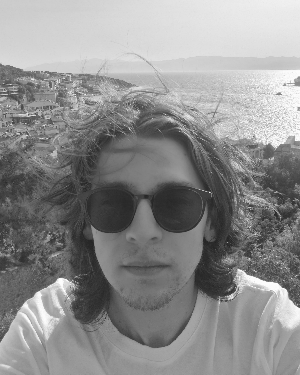
\includegraphics[width=1in,height=1.25in,clip,keepaspectratio]{author_ozcan.png}}]{Emre Özcan}
Senior Computer Engineering student at Manisa Celâl Bayar University
specializing in embedded systems, low-level programming and library development.
Skilled in clean code practices and first principles of computer science.
\end{IEEEbiography}

\begin{IEEEbiography}[{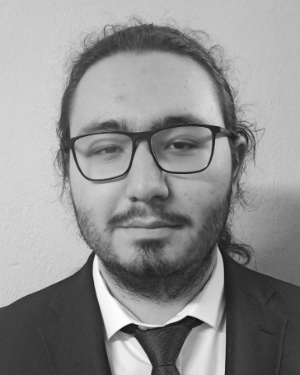
\includegraphics[width=1in,height=1.25in,clip,keepaspectratio]{author_gokce.png}}]{Eren Gökçe}
A 4th-year Computer Engineering student specializing in full-stack development
and Python programming.
Focused on building dynamic, user-centric applications and solving complex
challenges through innovative software
solutions.
Skilled in front-end and back-end technologies with a strong foundation in
engineering principles and a commitment to
impactful, efficient development.
\end{IEEEbiography}

\begin{IEEEbiography}[{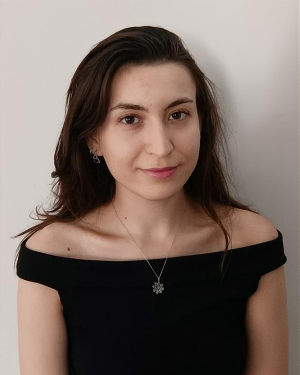
\includegraphics[width=1in,height=1.25in,clip,keepaspectratio]{author_uyar.png}}]{Melisa Uyar}
She was born on July 29, 2001, in Pinneberg, Germany.
She is currently a fourth-year computer engineering student at Manisa Celâl
Bayar University, specializing in back-end development.
She completed her internship at "BusinessUp," a performance marketing agency,
where she now works part-time.
At BusinessUp, she hones her skills in the Liquid programming language and
works as a junior full-stack developer.
\end{IEEEbiography}

\begin{IEEEbiography}{Muhammet Berk Can}
Motorcu çocuk
\end{IEEEbiography}

\begin{IEEEbiography}[{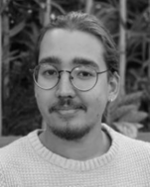
\includegraphics[width=1in,height=1.25in,clip,keepaspectratio]{author_ates.png}}]{Oğuz Anıl Ateş}
Was born in Uşak.
He graduated from Dursun Yalım Science High School in 2019.
He was accepted to the Computer Engineering department of Manisa Celâl Bayar
University (MCBU) in 2020.
He finished the preparatory year with a 97 GPA\@.
He continuous his fourth year of education in the field.
\end{IEEEbiography}

% if you will not have a photo at all:
%\begin{IEEEbiographynophoto}{John Doe}
%Biography text here.
%\end{IEEEbiographynophoto}

% insert where needed to balance the two columns on the last page with
% biographies
%\newpage

%\begin{IEEEbiographynophoto}{Jane Doe}
%Biography text here.
%\end{IEEEbiographynophoto}

% You can push biographies down or up by placing
% a \vfill before or after them. The appropriate
% use of \vfill depends on what kind of text is
% on the last page and whether or not the columns
% are being equalized.

%\vfill

% Can be used to pull up biographies so that the bottom of the last one
% is flush with the other column.
%\enlargethispage{-5in}

% that's all folks
\end{document}
